\chapter{Introduction}%
\label{CH:INTRODUCTION}

This thesis found a place inside the big and ambitious topic of motion planning, decision making, and control of
highly nonlinear robotic systems, with particular attention to the case of quadrotor flight platforms.
In this context, we aim to discuss and review the main problems which arise when approaching this field and try to
contribute by proposing novel solutions enabling the possibility to safely use these kinds of robots in humans' everyday life.
In the next chapters, we follow a tight golden line that allows touching each aspect of this field starting from the
used hardware, to the problem of mapping and localisation, ending with the motion planning, obstacle avoidance, and
advanced control techniques that make the robot acts safely in any conditions.
This chapter unfolds as follows, in~\secref{SEC:MOTIVATIONS} and~\secref{SEC:DRONE-CONTEST} we briefly analyse the motivations
behind this work, with an eye to the proposed project where the Ph.D. has been developed. In~\secref{SEC:HARDWARE-PLATFORM}
we describe the used UAV hardware, pointing out its sensing capabilities and the main challenges that emerge from its usage in
cluttered environments, finally in~\secref{SEC:CONTRIBUTIONS} we recap the main contributions of this dissertation.

%----------------------------------------------------------------------------------------
\section{Motivations}%
\label{SEC:MOTIVATIONS}
In the last decades, we saw a soaring interest in autonomous robots boosted not only by academia and industry, but also
by the ever increasing demand from civil users.
As a matter of fact, autonomous robots are fast spreading in all aspects of human life, we can see them clean houses,
navigate through city traffic, or harvest fruits and vegetables.
This trend is motivated by the fact that autonomous robots can assist humans in a plethora of daily activities
ranging from transportation and surveillance, to handling heavy loads and inspection.
In particular, UAVs can perform aerial inspection of industrial facilities or hazardous areas~\cite{nikolic2013uav},
surveillance and monitoring of conurbations~\cite{faigl2018surveillance}, crowded public places and warfare zones.
The automatisation of such activities can improve their quality, efficiency, and effectiveness, especially when performed by 
robots designed to use the most advanced technologies in analyzing and understanding the surrounding environment, such as
LiDAR laser scanners~\cite{marder2010office}, RGB-D and thermographic cameras~\cite{laguela2015aerial},
event-based cameras~\cite{vidal2017hybrid}, and others more.
Offloading error-prone, and potentially dangerous activities to robots that can automatically cope with them also
increases the quality of life for the human operators. In this respect, UAVs can contribute to preventing critical
situations and optimizing the management of urban environments~\cite{viragh2016self, villa2016overview}, 
performing search and rescue missions in hazardous scenarios~\cite{azzollini2021uav}, performing film shooting
in dangerous areas~\cite{huang2018act}, and monitoring cultivated fields~\cite{tsouros2019review}.
In order to perform the aforementioned tasks, the UAV platform must be endowed with a high level of onboard
intelligence that process the information gathered by the carried sensors and take real-time decisions.
Taking decisions is not the only workload that the onboard intelligence must sustain, as the UAV is also required
to fly smoothly without colliding and often mapping and memorising the explored environment. 
Almost all commercial drones already exhibit unprecedented and sophisticated skills such as obstacle avoidance~\cite{hrabar2011reactive},
simultaneous localisation and mapping~\cite{engel2014lsd}, path planning~\cite{ok2013path},
visual-interial odometry~\cite{forster2014svo}, and object tracking~\cite{mueller2016persistent}.
The major limitations of such robotic platforms lie in the limited payload that can carry, in their costs, and in the limited
autonomy due to finite battery capability. Nowadays, industries try to overtake these problems by designing very oversized
structures able to carry a large variety of sensors and very big batteries that can benefit from a very high autonomy.
This solution is not resolutive at all since it limits the UAVs field of application to very large environments, without containing
their cost and making their use unsafe for human operators.
For this reason researchers start to develop new algorithms able to run even on resource constrained platforms both in terms of
computation capabilities and limited types of endowed sensors, focusing especially on very cheap sensors and hardware.
The possibility to use a limited number of sensors allowed to scale a lot the UAVs size, while the implementation of new efficient
algorithms, performing the same task in lower time, allowed for lower autonomy.
In this respect, a new wave of innovation in aerial robotics is rapidly soaring: the miniaturization of vehicles~\cite{wood2012progress, floreano2015science, graule2016perching}.
Insect-scale autonomous UAVs can extend the applicability of flying robotic-helpers, making them even more pervasive in everyday life.
Thanks to their small form-factor, they can reach places otherwise inaccessible and increase the safety of operations in human-populated and indoor environments.
Although the field of nano- and pico-size UAVs is nowadays very widespread, the available algorithms are not mature enough to cope with
the limited resources and sensor data available onboard of these small platforms.
Besides that, a second big problem is related to the robustness of the adopted solutions as often require fine-tuning procedures to
be really effectiveness.
In this respect, the focus of this thesis lies on reviewing and discussing current state-of-the-art solutions to the problem of motion planning and control
specially tailored for autonomous aerial vehicles, then we aim to propose a bunch of new robust approaches focused on minimising the required
computational load with an eye to their flexibility and applicability in a wide range of different environments.

%----------------------------------------------------------------------------------------
\section{The Leonardo Drone Contest}%
\label{SEC:DRONE-CONTEST}
%%%%%%%%%%
\begin{figure}[!t]
	\centering
	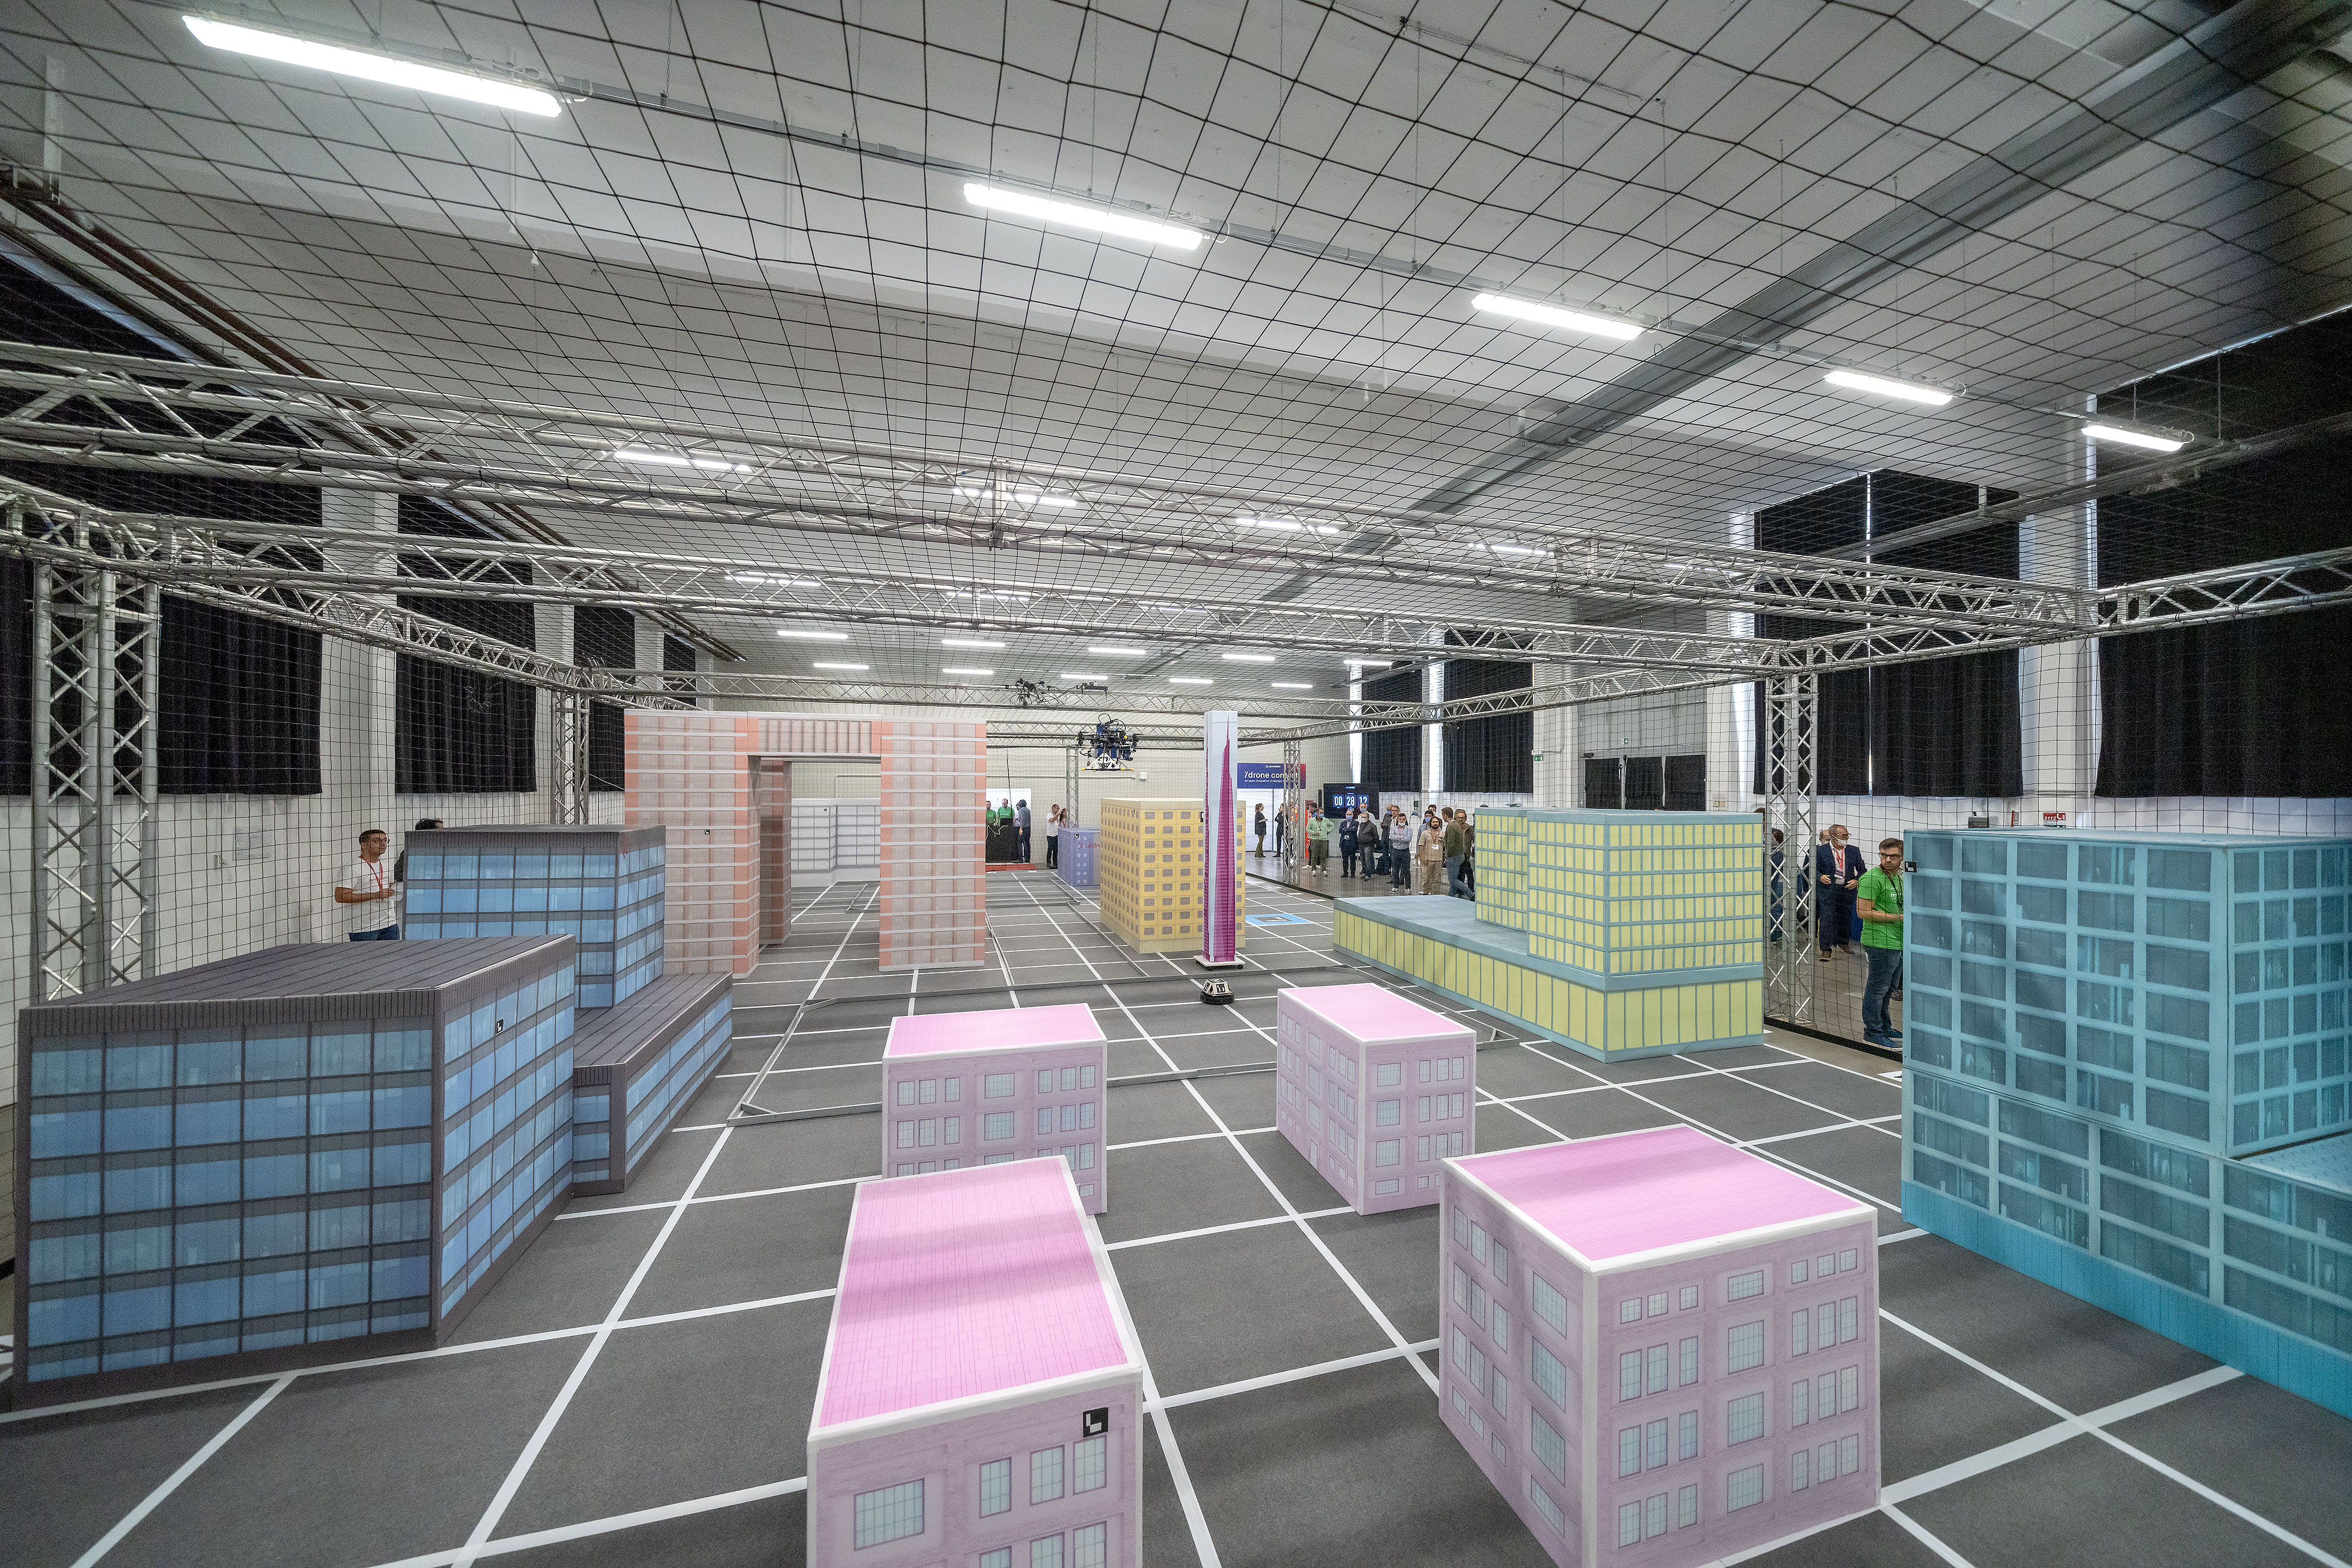
\includegraphics[width=1.\textwidth]{Figs/Chapter1/leonardo_map.jpg}
	\caption{Snapshot of the synthetic environment used during the Leonardo drone contest.}
	\label{FIG:LEONARDO-MAP}
\end{figure}
%%%%%%%%%%

The project behind the study which lead to the development of this dissertation consists of a drone competition
proposed by Leonardo S.p.A. to encourage the research in the field of autonomous flight robots.
The proposed contest completed five different Italian universities that developed five fully autonomous drones able to navigate
and explore a completely unknown environment and perform landing or inspection operations inside that area.
Leonardo builds a synthetic scenario mimicking an urban canyon of $20 \times 10 \times 3$ meters (see~\figref{FIG:LEONARDO-MAP})
to test the proposed solutions in three different application scenarios of increasing complexity. In the following,
we briefly report a description of the three proposed challenges, one for each Ph.D. study year.
\begin{itemize}
    \item[] \emph{The first year challenge.}\\
    In the first proposed challenge, the autonomous UAV was required to navigate and explore as fast as possible a completely unknown
    environment with the twice objective to generate a complete and precise map, and find out a set of ten ArUco markers~\cite{garrido2014automatic}
    scattered inside the environment. The UAV then had to perform a precise sequence of landing and takeoff actions on the detected markers.
    \item[] \emph{The second year challenge.}\\
    In the second challenge, the autonomous UAV was required to localise itself inside a previously mapped area, and to explore the
    environment to search for an autonomous ground agent moving randomly through the obstacles. Then the UAV had to track the found
    agent for a fixed amount of time without losing its sight, reading and recognizing an alphanumerical sequence printed on the chased robot.
    The read string contained the sequence of landing that the UAV was required to perform.
    The UAV had to collaborate with an external surveillance camera for better performing both the tasks of localisation and intrude finding.
    \item[] \emph{The third year challenge.}\\
    In the third proposed challenge, the autonomous UAV was required to localise itself inside a previously mapped area,
    and to explore the environment to search for an autonomous ground agent moving randomly through the obstacles.
    During such an exploration procedure, the UAV had to avoid unmapped static obstacles that suddenly appeared inside the area.
    Then the UAV had to track the found ground robot for a fixed amount of time without losing its sight.
    Once done that, a human operator committed a sequence of landing or buildings inspection actions that the drone was required to perform.
\end{itemize}
As the reader can conceive, the proposed challenges cover almost all the aspects of the big field of autonomous navigation.
As a matter of fact, the developed platform must be able to localise itself, map the surrounding environment, plan safe paths or trajectories
through already mapped obstacles, and react to the unknown by replanning previously established safe paths.
Moreover, the UAV must be able to reliably chase moving objects, explore unknown environments, performing precise landings, and
plan highly informative trajectories to perform building inspection.
The list of required capabilities is not short, and for each of them a deeper study of the current state-of-the-art had been carried out.
In this thesis, the reader will find a brief review of most of the aforementioned topics along with a description of how each
problem has been solved in the \emph{Leonardo drone contest}.

%----------------------------------------------------------------------------------------
\section{The Benchmark Platform}%
\label{SEC:HARDWARE-PLATFORM}
%%%%%%%%%%
\begin{figure}[!t]
	\centering
	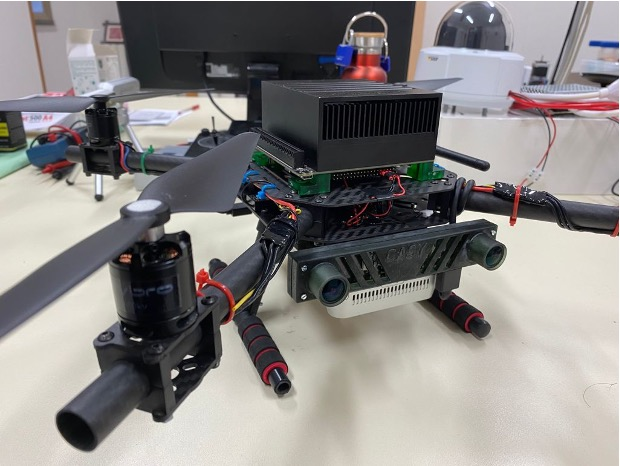
\includegraphics[width=0.8\textwidth]{Figs/Chapter1/drone.pdf}
	\caption{Developed drone used during the Leonardo drone contest.}
	\label{FIG:DRONE-PLATFORM}
\end{figure}
%%%%%%%%%%
The quadcopter deployed during the Leonardo drone contest (see~\figref{FIG:DRONE-PLATFORM}) is a commercial drone 
\emph{Holybro X500} customized for our particular application, of dimension $750 \times 750 \times 370$ millimeters,
with a weight of $1530$ grams, and is powered with a $6200$ \emph{mAh} battery. The quadcopter is endowed with a
\emph{Pixhawk 4}~\cite{meier2011pixhawk} computational unit running the \emph{PX4 Autopilot}~\cite{meier2015px4}.
Besides this unit, the UAV carries a \emph{Jetson Xavier NX} companion computer responsible for running all
control, planning, localisation, and perception algorithms. All the developed algorithms are tightly integrated
inside a ROS network and exchange messages with the Pixhawk computational unit via \emph{MAVLink} interface~\cite{koubaa2019micro}.
The chosen sensor suite consists of a $9$-axis Inertial Measurement Unit (IMU), inclusive of accelerometers, gyroscopes, and
magnetometers, and two stereo cameras pointing backward and forward, respectively.
The sensor suite is intentionally poor and GPS free, to let the robot navigate in GPS-denied environments such as indoor areas,
and to keep the overall platform cost low.
The overall quadcopter comprising of all sensors and computational units weights $1960$ grams and has a payload of $500$ grams
at $60\%$ of throttle.

%----------------------------------------------------------------------------------------
\section{Contributions}%
\label{SEC:CONTRIBUTIONS}
The contribution of this thesis is twofold, on one side it is meant to present and describe a practical software solution
to the problem of autonomous navigation in unknown, or partially known, environments.
Such a solution has been extensively tested and validated in real scenario experiments and presented as a final UAV architecture
during the Leonardo drone contest (see~\secref{SEC:DRONE-CONTEST}).
The proposed solution is often built upon existing stat-of-the-art algorithms properly modified and robustified to cope with
the strong real-time and reliability requirements imposed by the contest.
A reader only interested in the aforementioned architecture hardly finds a smooth discussion of all software modules.
The thesis presentation is in fact intentionally left unstructured, although the chapters sequence remark the
localisation-planning-control pipeline, each chapter decomposes the problem at hand and in addition to providing a
practical solution, it aspires to present innovative ideas and contributions.
This is the second contribution of this thesis that, for each aspect of autonomous navigation, tries to improve
the current state-of-the-art by leveraging on solutions which reduce, or eliminate, the major limitations of the
most popular algorithms.

%------------------------------------------------